\documentclass{tufte-handout}

%\geometry{showframe}% for debugging purposes -- displays the margins

\usepackage{amsmath}

% Set up the images/graphics package
\usepackage{graphicx}
\setkeys{Gin}{width=\linewidth,totalheight=\textheight,keepaspectratio}
\graphicspath{{graphics/}}

\title{Gluconeogenesis}
\author{}
\date{}  % if the \date{} command is left out, the current date will be used

% The following package makes prettier tables.  We're all about the bling!
\usepackage{booktabs}

% The units package provides nice, non-stacked fractions and better spacing
% for units.
\usepackage{units}

% The fancyvrb package lets us customize the formatting of verbatim
% environments.  We use a slightly smaller font.
\usepackage{fancyvrb}
\fvset{fontsize=\normalsize}

% Small sections of multiple columns
\usepackage{multicol}

% Provides paragraphs of dummy text
\usepackage{lipsum}

% These commands are used to pretty-print LaTeX commands
\newcommand{\doccmd}[1]{\texttt{\textbackslash#1}}% command name -- adds backslash automatically
\newcommand{\docopt}[1]{\ensuremath{\langle}\textrm{\textit{#1}}\ensuremath{\rangle}}% optional command argument
\newcommand{\docarg}[1]{\textrm{\textit{#1}}}% (required) command argument
\newenvironment{docspec}{\begin{quote}\noindent}{\end{quote}}% command specification environment
\newcommand{\docenv}[1]{\textsf{#1}}% environment name
\newcommand{\docpkg}[1]{\texttt{#1}}% package name
\newcommand{\doccls}[1]{\texttt{#1}}% document class name
\newcommand{\docclsopt}[1]{\texttt{#1}}% document class option name

\begin{document}

\maketitle% this prints the handout title, author, and date

\begin{abstract}
\noindent Glucose is not an essential nutrient, and can be generated from a variety of precursors including glycerol, lactate and amino acids.  This is important because several tissues, including the brain, are highly dependent on glucose levels.  As such, the body maintains blood glucose levels in a very narrow range, and gluconeogensis is essential to ensuring glucose is available in the blood.  This unit will describe the function and regulation of gluconeogenesis including its regulation by internal and external signals.  For more details on gluconeogenesis, refer to Chapter 17 of Biochemistry: A Short Course\cite{Berg2015} and Chapter 10 of Lippincott's Illustrated Reviews: Biochemistry\cite{Ferrier2017}, both on reserve.
\end{abstract}

\tableofcontents
\pagebreak
\section{Learning Objectives}

\begin{itemize}
\item Describe the tissues where gluconeogenesis occurs and the key enzymatic determinants of this specificity.
\item Explain the major precursors of gluconeogenesis, including where they are derived from and at what step they integrate.
\item Evaluate how the flow of each these precursors is regulated differently, dependent on where they enter the gluconeogenic pathway.
\item Analyse the energetic costs of gluconeogenesis, given the precursor substrate.
\item Describe how chronic activation of gluconeogenesis results in ketone body production from the liver.
\item Understand the importance of the Cori and Cahill cycles in recycling waste products back to glucose.
\end{itemize}

\section{The Importance in Maintaining Blood Glucose Levels}

While many tissues we focus on in this course can use a variety of substrates for fuel, such as amino acids, glucose or lipids some tissues are highly dependent on glucose.  Among these are the brain, and red blood cells.  Adding to this problem, neurons are very poor at storing glucose as glycogen, which means they need a constant infusion of glucose from the blood to maintain their function.  While the brain is generally only 2\% of the mass of a human, it consumes around 20\% of the glucose in the body \citep{Erbsloh1958}.  Even individuals who consume extremely low carbohydrate diets are able to maintain their blood glucose near the normal range\sidenote{While individuals on ketogenic diets still use a lot of glucose for brain function, there is evidence that in those individuals the brains can adapt to use ketone bodies as an energy source as well.  We will discuss this in the lectures on lipid oxidation later on in the semester.} \citep{Bueno2013}.  The ability to maintain blood glucose, with limited dietary carbohydrate ingestion in the primary role of gluconeogenesis.

\section{Gluconeogenesis Primarily Occurs in the Liver and Kidneys}

The primary glucose producing tissues are the liver and the kidneys.  The molecular determinant of this is the presence of the enzyme Glucose-6-Phosphatase which catalyzes the removal of phosphate from Glucose-6-Phosphate, allowing it to be exported from the cell.  While gluconeogenic substrates can become converted to Glucose-6-Phosphate through similar pathways described below, the final phosphate removal and release of glucose only occurs in cells with this enzyme.

\newthought{Glucokinase plays an important role in this process.}  If you recall from the lecture on glycolysis, the biochemistry of the Glucokinase is an important part of this regulation.  Mscle and adipose tissues have hexokinase, which is very efficient at phosphorylating even low concentrations of Glucose. Glucokinase, which is present in the liver, has very low kinetic efficiency at low glucose concentrations.  This means that when glucose levels are low in the blood, Glucokinase will be inactive and Glucose-6-Phosphate dephosphorylation will not be reversed.

\section{Gluconeogenic Substrates}

There are several substrates that can be converted into glucose as illustrated in Figure \ref{fig:gluconeogenic-substrates}.  The first thing to notice is how similar the ovelap of this pathway is to glycolysis.  Most of the reactions described in glycolysis are reversed in gluconeogenesis, and are catalyzed by the same enzymes.  As you read about these reactions, consider that the biochemical step at which a gluconeogenic substrate enters the pathway dictates what sites of regulation are essential to the control of its metabolism.  

\begin{marginfigure}
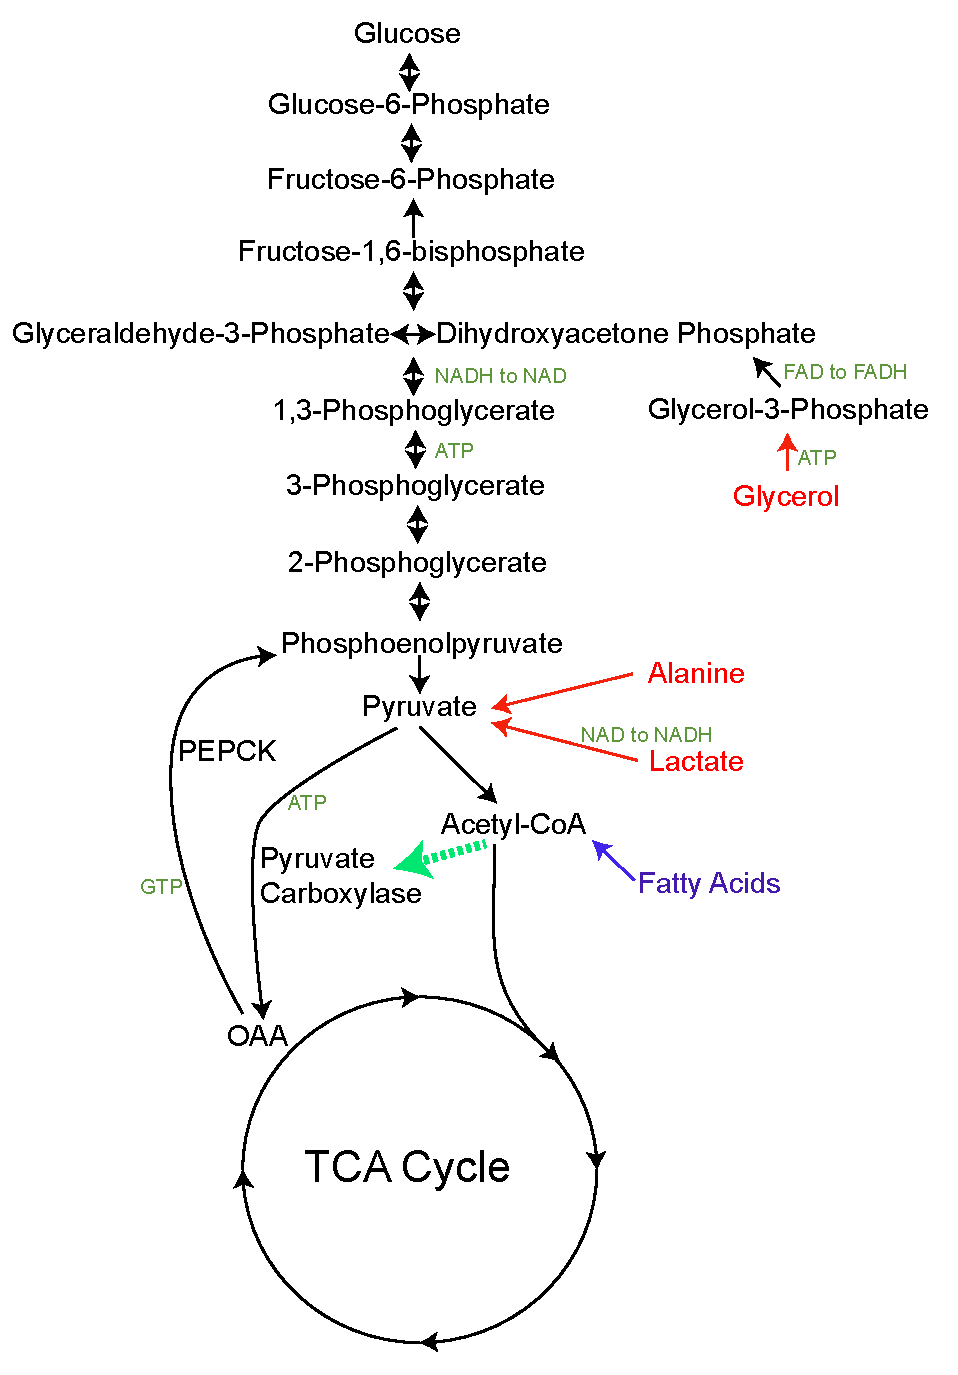
\includegraphics{figures/gluconeogenic-substrates.pdf}
\caption{Schematic of gluconeogenesis.  Red indicates key gluconeogenic substrates while green indicates energy consuming or generating steps.}
\label{fig:gluconeogenic-substrates}
\end{marginfigure}

\subsection{Glycerol}

Glycerol is derived from the breakdown of triglycerides and is increased during lipolysis.  That process releases both glycerol and free fatty acids, both of which traffic to the liver.  While fatty acids (shown in blue in Figure \ref{fig:gluconeogenic-substrates}) are \emph{unable} to be converted to glucose, they play a role in regulating Pyruvate Carboxylase, described in a later section.  Glycerol on the other hand becomes activated by phosphorylation, then is converted into DHAP.  DHAP and GA3P are combined by Aldolase into Fructose-1,6-bisphosphate, which is then dephosphorylated by Fructose bisphosphatase\sidenote{FBPase is a key point of gluconeogenic regulation discussed in detail later}.

\subsection{Lactate and the Cori Cycle}

Lactate, the product of anaerobic glycolysis can be interconverted back to pyruvate via the reversible actions of Lactate Dehydrogenase.  This is an important inter-organ cycle called the Cori Cycle\sidenote{Or the Lactic Acid Cycle.  This is named after Carl and Gery Cori who won the Nobel Prize in Medicine or Physiology for this and her work on glycogen metabolism.  Gerty Cori was the first woman to win the Nobel Prize in Medicine or Physiology.}.  This cycle involves the anaerobic breakdown of glucose to lactate in the muscle, followed by its re-synthethis back to glucose in the liver.  This re-formed glucose now travels back to the muscle.  Overall this cycle consumes two ATP molecules\sidenote{Do the math!} so is energy consuming, but is an important way to ensure that the muscle has sufficient glucose available for anaerobic metabolism.

\subsection{Alanine and other Amino Acids}

Several amino acids can be converted back to glucose.  This class of amino acids is known as the \emph{glucogenic} amino acids and includes Alanine, Arginine, Aspartate, Asparagine, Cysteine, Glutamate, Glutamine, Glycine, Histidine, Methionine, Proline Serine and Valine.  The other amino acids that cannot be converted to glucose are known as ketogenic amino acids\sidenote{We will cover this in more detail in the amino acid catabolism lectures}.  The catabolic routes of these amino acids vary but the most important of them is Alanine. As we discussed regarding the fates of Pyruvate, Alanine and Pyruvate can be inter-converted via the actions of Alanine Aminotransferase (ALT):


\begin{equation}\label{eq:alt}
Alanine + \alpha - Ketoglutarate \leftrightarrow Glutamate + Pyruvate
\end{equation}

This enzyme is important for making Alanine (for example when levels are low and Pyruvate levels are high), but also can regenerate pyruvate for gluconeogenesis.  As shown in Figure \ref{fig:gluconeogenic-substrates} the conversion of Pyruvate to Phosphoenolpyruvate\sidenote{This is the inverse of the Pyruvate Kinase reaction that was important for glycolysis.} is not a simple reversible reaction.  Instead, for Pyruvate to undergo gluconeogenesis, it first must be carboxylated to oxaloacetic acid (OAA) by Pyruvate Carboxylase and then converted back to Phosphoenolpyruvate by the enzyme Phosphoenolpyruvate carboxykinase (PEPCK).  Both of these enzymes are important sites of regulatory control. It is important to not at this stage that (absent the balancing influx of Alanine) activation of PEPCK is highly cataplerotic.  It removes TCA cycle intermediates (OAA) and pushes them towards gluconeogenesis.  This means that gluconeogenesis can occur at a cost of TCA cycle efficiency, since when OAA is depleted, Acetyl-CoA cannot enter the TCA cycle for energy production\sidenote{This is the main reason why very low carbohydrate diets result in ketone body production.  Gluconeogenesis depletes OAA, and Acetyl-CoA is converted into ketone bodies because they cannot enter the TCA cycle}.

\newthought{Alanine reconversion to glucose is known as the Cahill Cycle\sidenote{Also known as the Glucose-Alanine cycle.}}  Similar to the Cori cycle, the cycle of Alanine release from muscle, conversion to glucose and then return to blood glucose is an important inter-organ metabolic loop.  When muscle is broken down, Alanine is released and can be converted by the liver back into glucose for fuel.  This is more costly than the Cori cycle, because Urea must be removed from Glutamate\sidenote{Again, this will be discussed later when we talk about amino acid catabolism.}.  This cycle uses 4 ATP equivalents for the Urea cycle and 11 ATP molecules for Gluconeogenesis, so requires a lot of energy from the liver.

\section{Energetic Demands of Gluconeogenesis}

Gluconeogenesis is generally energetically costly.  It requires a varible number of ATP molecules depending on the substrate\sidenote{Try to calculate this yourself for each of the substrates.}.  The energy consuming steps, shown in Figure \ref{fig:gluconeogenic-substrates} are Pyruvate Carboxylase (one ATP), PEPCK (one GTP\sidenote{This is equivalent to one ATP}), and Phosphoglycerate Kinase (1 ATP).  Since at the Aldolase step, two three carbon precursors (GA3P and DHAP) are combined, this means that to make one molecule of glucose you need to follow this pathway twice.  That means that to go from Pyruvate to Glucose you need 2 x 3 ATP equivalents plus two NADH equivalents (at the Glyceraldehyde Dehydrogenase step).  Since each NADH is equivalent to 2.5 ATP molecules, gluconeogenesis from Pyruvate consumes 11 ATP equivalents per glucose produced.  A summary for the main gluconeogenic substrates are shown in Table \ref{tab:gluconeogenesis-energetics}.

\begin{table}
\centering
\caption{Gluconeogenic energy use in terms of ATP equivalents.}
\label{tab:gluconeogenesis-energetics}
\begin{tabular}{cccc}
\hline
\textbf {Substrate} & \textbf{Gluconeogenesis}  & \textbf{Urea Cycle} & \textbf{Total}\\
\hline
Glycerol & +1 & 0 & +1\\
Lactate & -6 & 0 & -6 \\
Alanine & -11 & -4 & -15\\
\hline
\end{tabular}
\end{table}

\section{Key Regulatory Steps in Gluconeogenesis}

Since it is counterproductive to have gluconeogenesis and glycolysis operating simulataneously the regulation of these pathways is largely reciprocal.  Generally when one pathway is activated, the other is inactivated.  In the case of gluconeogenesis, the key points of regulation are Pyruvate Carboxylase, PEPCK, FBPase and Glucose-6-Phosphatase/Glucokinase.  These are under a combination of acute (rapid and reversible, mainly allosteric) and chronic (slow and permanent, mainly transcriptional) control mechanisms. 

\subsection{Acute Regulation of Gluconeogenesis}

As we discussed in the TCA cycle lecture, Pyruvate Carboxylase is a key anaplerotic enzyme.  It is stimulated by Acetyl-CoA levels, to generate OAA from Pyruvate.  In terms of gluconeogenesis, recent research has highlighted a key role of fatty acid-derived Acetyl-CoA as promoting glucose production \cite{Perry2015}.  While fatty acids cannot directly be converted into glucose, this is one mechanism by which they induce gluconeogenesis.  This has important consequences for understanding the relationships between the regulation of lipolysis on glucose production.

\newthought{The second major site of acute control is at the FBPase step.}  Fructose-2,6-bisphosphatase is the opposite function of PFK2, discussed in detail in the glycolysis lecture. In fact, they are the same polypeptide, comprising a bifunctional enzyme.  FBPase will remove the phosphate from F26bP, depleting that important allosteric activator of PFK1\sidenote{F26bP is also an inhibitor of FBPase1, so its removal activates gluconeogenesis}. The same PKA-dependent phosphorylation that that reduced PFK2 activity activates FBPase2 activity resulting in less F26bP and F16bP continue towards glucose.  In addition to the effects of F26bP, FBPase1 is also inhibited by AMP.  Since gluconeogenesis is so energy consuming, this regulatory step ensures that ATP is sufficient for gluconeogneesis to occur.  A comparason of FBPase1 and PFK1 are shown in Table \ref{tab:fbpase-pfk}.  More details about FBPase regulation can be found in this review: \citet{Okar2001}. 

\newthought{PKA, activated by Glucagon or Epinephrine promotes gluconeogenesis in the liver}.  By inactivating PFK2 and activating FBPase2, PKA drives glucose production from precursor molecules in the liver.  This, along with the breakdown of glycogen provides muscles and other tissues with glucose in times of need.  Gluconeogenesis is slower and more costly than glycogenolysis, but is able to use a wider variety of pools to make glucose.

\begin{margintable}
\centering
\caption{PFK1 and FBPase1 Regulation}
\label{tab:fbpase-pfk}
\begin{tabular}{ccc}
\hline
\textbf {Regulator} & \textbf{PFK1}  & \textbf{FBPase1} \\
\hline
F26bP & Activates & Inactivates\\
AMP & Activates & Inactivates \\
ATP & Inactivtes & - \\
Citrate & Inactivates & - \\
PKA & Inactivates & Activates\\
\hline
\end{tabular}
\end{margintable}

\subsection{Transcriptional Regulation of Gluconeogenesis}

In contrats to PKA's effects activating gluconeogenesis, insulin potently suppresses the production of glucose.  Since insulin is elevated in response to elevations in glucose, this suppression is a major part by which insulin reduces blood glucose\sidenote{The others being stimulation of glucose uptake and glycogenesis}.  One mechanism by which this is thought to occur is through transcriptional regulation, largely through the transcription factor FOXO.  Insulin promotes the Akt-dependent phosphorylation of FOXO, which removes it from the nucleus, rendering it inactive.  Several key gluconeogenic genes are FOXO targets including PEPCK and G6Pase.  This means that when insulin inhibits FOXO function, the transcription of those genes is markedly reduced.  More information about the role of FOXO can be found in \citet{Barthel2005}.

\newthought{Cortisol is another gluconeogenic hormone.}  By binding to its nuclear hormone receptor, glucocorticoids such as cortisol can promote the transcription of Pyruvate Carboxylase, PEPCK and G6Pase.  You can think of this as the opposite of the effects of insulin.  By synthesizing more of these rate limiting enzymes, cortisol can promote glucose produciton and make glucose available to the rest of the body during times of stress.  Notably, glucocorticoid-induced hyperglycemia is an important result of Cushing's disease\sidenote{Overproduction of cortisol by the adrenal gland, often associated with pituitary or adrenal tumors.} or prescription glucocorticoids such as predinosone or cortisone.

\section{Consequences of Unrestrained Gluconeogenesis}

While gluconeogenesis is essential to maintaining blood glucose levels in times of glucose deprivation, it is a key hallmark of both Type 1 and Type 2 diabetes.  Insulin's ability to suppress gluconeogenesis is either not present (in type 1) or impaired (in type 2 diabetes).  Diabetics therefore tend to have over-active gluconeogenesis, which results in elevated blood glucose.  Gluconeogenesis is therefore a key pharmacological and nutritional target for controlling blood glucose in diabetes, which now affects more than 29 million Americans, with another 86 million considered at risk\cite{CentersforDiseaseControl2016}.




\bibliography{library}
\bibliographystyle{plainnat}

\end{document}
